\documentclass{beamer}
\usepackage[utf8]{inputenc}
\usetheme{Madrid}
\usecolortheme{default}
\usepackage{amsmath,amssymb,amsfonts,amsthm}
\usepackage{txfonts}
\usepackage{tkz-euclide}
\usepackage{listings}
\usepackage{adjustbox}
\usepackage{array}
\usepackage{tabularx}
\usepackage{gvv}
\usepackage{lmodern}
\usepackage{circuitikz}
\usepackage{tikz}
\usepackage{graphicx}

\setbeamertemplate{page number in head/foot}[totalframenumber]

\usepackage{tcolorbox}
\tcbuselibrary{minted,breakable,xparse,skins}



\definecolor{bg}{gray}{0.95}
\DeclareTCBListing{mintedbox}{O{}m!O{}}{%
  breakable=true,
  listing engine=minted,
  listing only,
  minted language=#2,
  minted style=default,
  minted options={%
    linenos,
    gobble=0,
    breaklines=true,
    breakafter=,,
    fontsize=\small,
    numbersep=8pt,
    #1},
  boxsep=0pt,
  left skip=0pt,
  right skip=0pt,
  left=25pt,
  right=0pt,
  top=3pt,
  bottom=3pt,
  arc=5pt,
  leftrule=0pt,
  rightrule=0pt,
  bottomrule=2pt,
  toprule=2pt,
  colback=bg,
  colframe=orange!70,
  enhanced,
  overlay={%
    \begin{tcbclipinterior}
    \fill[orange!20!white] (frame.south west) rectangle ([xshift=20pt]frame.north west);
    \end{tcbclipinterior}},
  #3,
}
\lstset{
    language=C,
    basicstyle=\ttfamily\small,
    keywordstyle=\color{blue},
    stringstyle=\color{orange},
    commentstyle=\color{green!60!black},
    numbers=left,
    numberstyle=\tiny\color{gray},
    breaklines=true,
    showstringspaces=false,
}


\title 
{1.3.7}
\date{August 27,2025}


\author 
{Manohar-AI25BTECH11028}



\begin{document}


\frame{\titlepage}
\begin{frame}{Question}
Find the coordinates of the  vertex $A$ of an ABCD parallelogram whose three vertices are given as B$\brak{0,0}$,C$\brak{3,0}$, and D$\brak{0,4}$.
\end{frame}





\begin{frame}{Equation}
Given points,
\begin{align}
    \vec{B}=\begin{myvec}{0\\0}\end{myvec}
    \vec{C}=\begin{myvec}{3\\0}\end{myvec} \vec{D}=\begin{myvec}{0\\4}\end{myvec}
\end{align}

we can use the parallelogram property that if ABCD be a parallelogram ,
\begin{align}
\vec{B}-\vec{A}=\vec{C}-\vec{D
}.\\
\end{align}
\end{frame}
\begin{frame}{Theoretical Solution}

In a paralleleogram,
\begin{align}
\vec{A} = \vec{B} + \vec{D} - \vec{C}\\
        = \myvec{0\\0} + \myvec{0\\4} - \myvec{3\\0}\\
= \myvec{-3\\4}
\end{align}
Therefore,
\begin{align}
    \vec{A}=\myvec{-3\\4}
\end{align}

\end{frame}


\begin{frame}[fragile]
    \frametitle{C Code}

    \begin{lstlisting}

#include<stdio.h>

int main() {
    int Bx=0, By=0, Cx=3, Cy=0, Dx=0, Dy=4;
    int Ax, Ay;

    // Formula: A = B + D - C
    Ax = Bx + Dx - Cx;
    Ay = By + Dy - Cy;

    printf("Coordinates of A: (%d, %d)\n", Ax, Ay);
    return 0;
}

    \end{lstlisting}
\end{frame}

\begin{frame}[fragile]
    \frametitle{Python Code}
    \begin{lstlisting}
    import numpy as np
import matplotlib.pyplot as plt

# Given vertices
B = np.array([0, 0])
C = np.array([3, 0])
D = np.array([0, 4])

# Compute A = B + D - C
A = B + D - C
print("Coordinates of A:", A)






    \end{lstlisting}
\end{frame}

\begin{frame}[fragile]
    \frametitle{Python Code}
    \begin{lstlisting}
    # Plot parallelogram
x_points = [A[0], B[0], C[0], D[0], A[0]]
y_points = [A[1], B[1], C[1], D[1], A[1]]

plt.plot(x_points, y_points, 'b-')
plt.scatter([A[0], B[0], C[0], D[0]], [A[1], B[1], C[1], D[1]], color='r')


    \end{lstlisting}
\end{frame}

\begin{frame}[fragile]
    \frametitle{Python Code}
    \begin{lstlisting}
     plt.text(A[0]-0.3, A[1]+0.2, 'A(-3,4)')
plt.text(B[0]-0.3, B[1]-0.3, 'B(0,0)')
plt.text(C[0]+0.2, C[1]-0.3, 'C(3,0)')
plt.text(D[0]-0.3, D[1]+0.3, 'D(0,4)')

plt.axis('equal')
plt.grid(True)


    \end{lstlisting}
\end{frame}


\begin{frame}[fragile]
    \frametitle{Python Code}
    \begin{lstlisting}


# Save before show
plt.savefig("/storage/emulated/0/matrix/Matgeo/1.3.7/figs/Figure_1.png", dpi=300, bbox_inches='tight')
plt.show()
    \end{lstlisting}
\end{frame}


\begin{frame}{Plot}
    \centering
    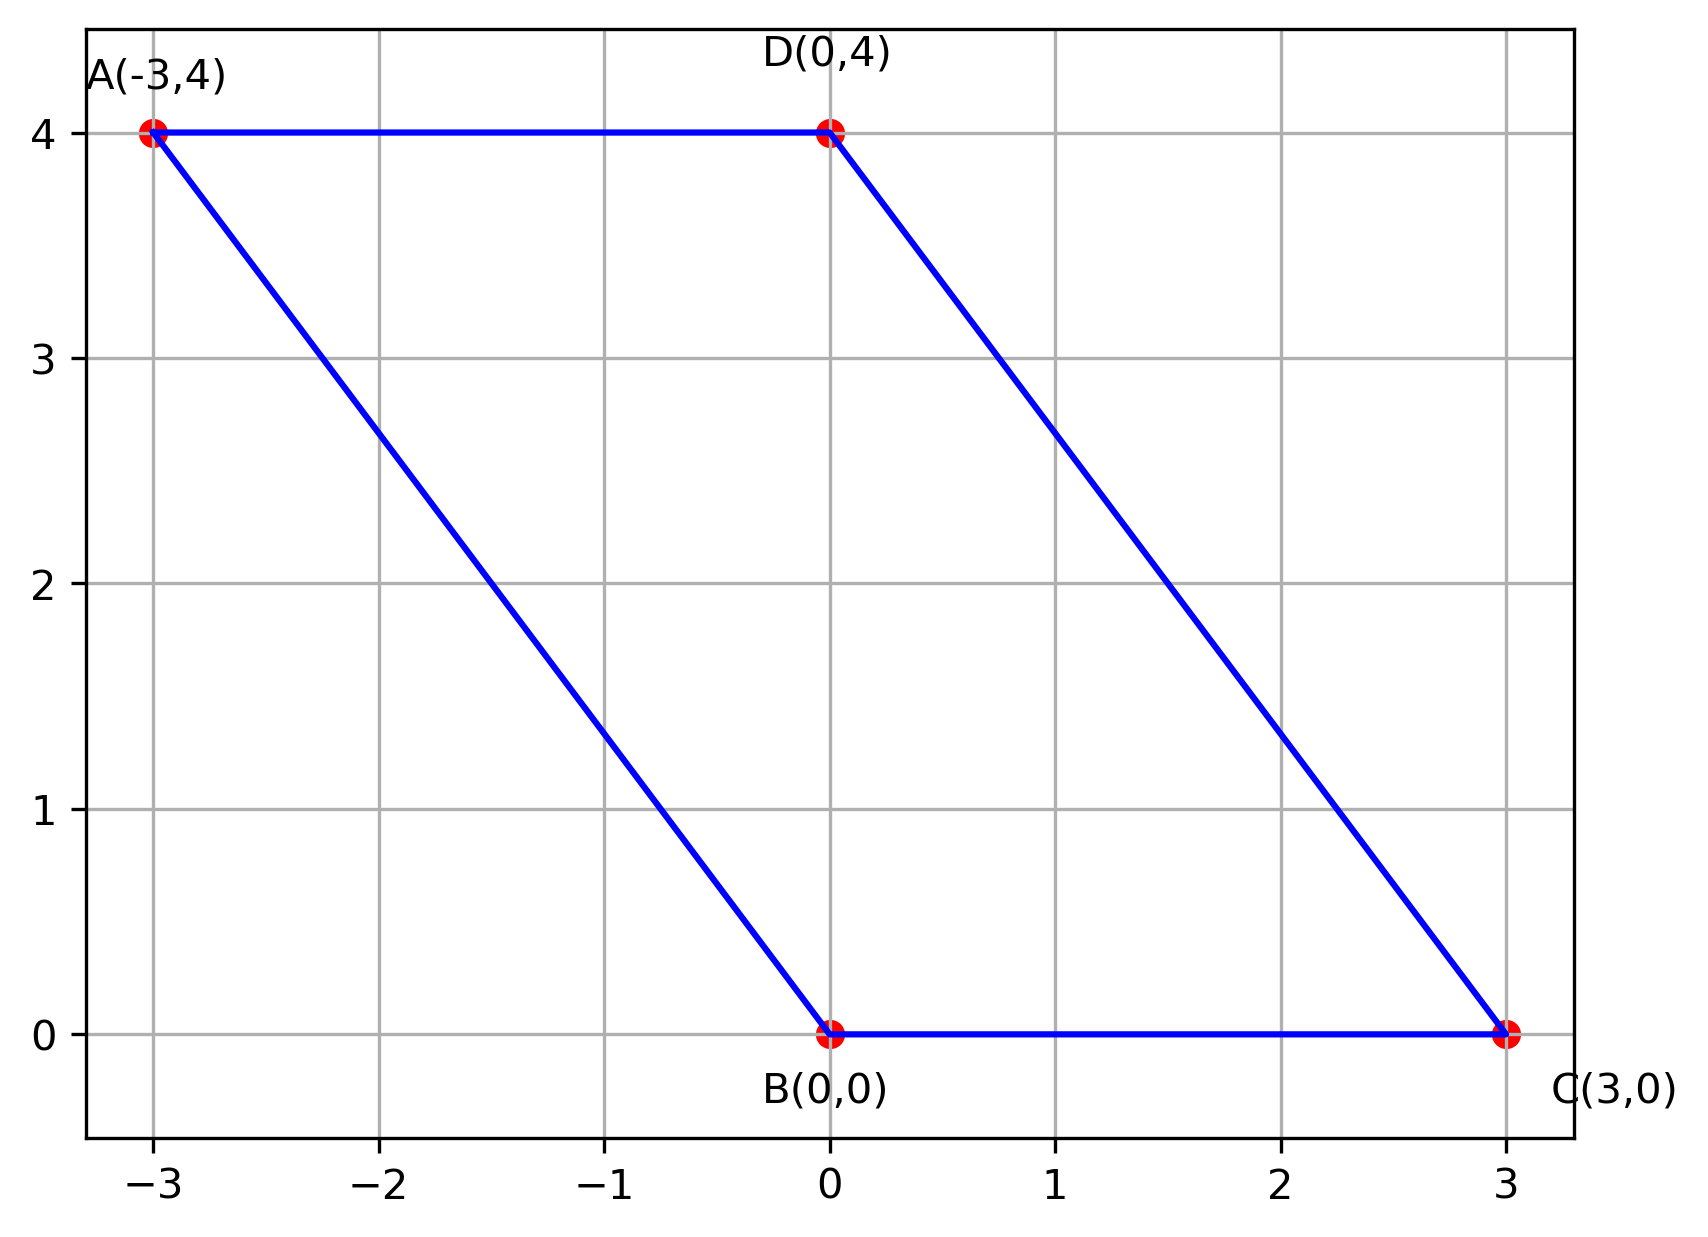
\includegraphics[width=\columnwidth, height=0.8\textheight, keepaspectratio]{figs/figure_1.png}     
\end{frame}


\end{document}
